\subsection{Modelo de datos conceptual}

El modelo de datos de la solución se fundamenta en un conjunto de entidades de negocio canónicas, sus relaciones y eventos, conforme a RT-02.13. Este modelo alimenta la matriz de trazabilidad que exige el numeral 17.1 de las Bases Técnicas del caso (cap. 17, p. 31), entregada en el Formulario T-12, y los contratos de integración (OpenAPI 3.1 y AsyncAPI 2.6 por módulo).

Las entidades principales son:

\begin{itemize}
  \item \textbf{Cliente.} Con RUT, razón social, canal (tradicional, food service, cadenas), crédito, georreferencia y estado de bloqueo. Eventos: creación, actualización y cambio de bloqueo.
  \item \textbf{Pedido.} Identificador UUID, preventista, cliente, líneas de detalle (SKU, cantidad, precio) y ciclo de vida (tomado $\rightarrow$ confirmado $\rightarrow$ preparado $\rightarrow$ despachado $\rightarrow$ entregado $\rightarrow$ rendido). Eventos: toma, confirmación, asignación de línea, despacho y evidencia de entrega.
  \item \textbf{SKU / Producto.} Con codificación GTIN/GS1, unidad, clasificación de temperatura, rangos térmicos (RF-09.01) y vida útil.
  \item \textbf{Lote.} Unidad de trazabilidad sanitaria identificada por GTIN y número de lote del proveedor, con vencimiento como atributo asociado. Cada movimiento interno la vincula con su unidad logística SSCC. Eventos: recepción, bloqueo, inicio de retiro sanitario y enlace con unidad logística.
  \item \textbf{Misión de preparación.} HHT, oleada, ubicación, unidades y ciclo de vida (descargada $\rightarrow$ ejecutada $\rightarrow$ cerrada).
  \item \textbf{Ruta / viaje.} Planificador, vehículo, conductor, ventanas, secuencia de entregas y geocercas.
  \item \textbf{Entrega.} Pedido, viaje, prueba de entrega (POD: firma, QR, fotografía), documentos DTE y efectivo. Eventos: evidencia, reintento y aprobación de rendición.
  \item \textbf{Documento tributario.} Factura, boleta, guía de despacho, folio del SII y acuse.
  \item \textbf{Envase retornable.} Canastillo o pallet, cliente, saldo y pérdida estimada del 14\% anual (Decisión 16.1 N\textdegree{} 10). Control por cuenta corriente por cliente, no por unidad identificada.
  \item \textbf{Sensor / registro térmico.} Dispositivo, lote o posición, temperatura y excursión térmica.
\end{itemize}

Los eventos usan verbos en pasado y son la base de los esquemas AsyncAPI. Toda escritura offline es idempotente por UUID (RT-02.06; Bases Técnicas Transversales, cap. 2, p. 7).

El almacenamiento se distribuye en quince dominios lógicos: BD\_INVENTARIO, BD\_PREVENTA, BD\_RUTAS (PostGIS), BD\_PREPARACION, BD\_REPARTO, BD\_COBRANZA\_FINANZAS, BD\_MAESTROS\_CONF, BD\_GOBIERNO\_ACCESO, BD\_CALIDAD\_TRAZABILIDAD, BD\_TELEMETRIA, BD\_EDI\_CANALMODERNO, BD\_BI\_GERENCIA, BD\_MAILS\_NOTIF, REDIS\_SESIONES\_CACHE y S3\_DOCS. El dominio de telemetría conserva la ingesta raw en DynamoDB y su serie consolidada en S3 Parquet y Redshift, procesada con Glue. Esta separación incluye bases transaccionales, almacenes analíticos, caché y objetos; no representa quince servidores físicos ni quince motores de base de datos independientes.

La Figura~\ref{fig:arql-18} relaciona las entidades principales con los módulos responsables y sus intercambios. Esta vista de dominio permite seguir la confirmación del pedido, la custodia del lote y la entrega sin duplicar el detalle de atributos, claves y cardinalidades del Subdocumento 5. Ese detalle se desarrolla en 5.1 y sus anexos; la separación de autoridad entre reserva comercial y retención física se explica en 5.2. La lectura conjunta permite responder de qué lote provino una unidad entregada y a qué clientes llegó un lote que debe retirarse.

\begin{anexohorizontal}
\begin{center}
  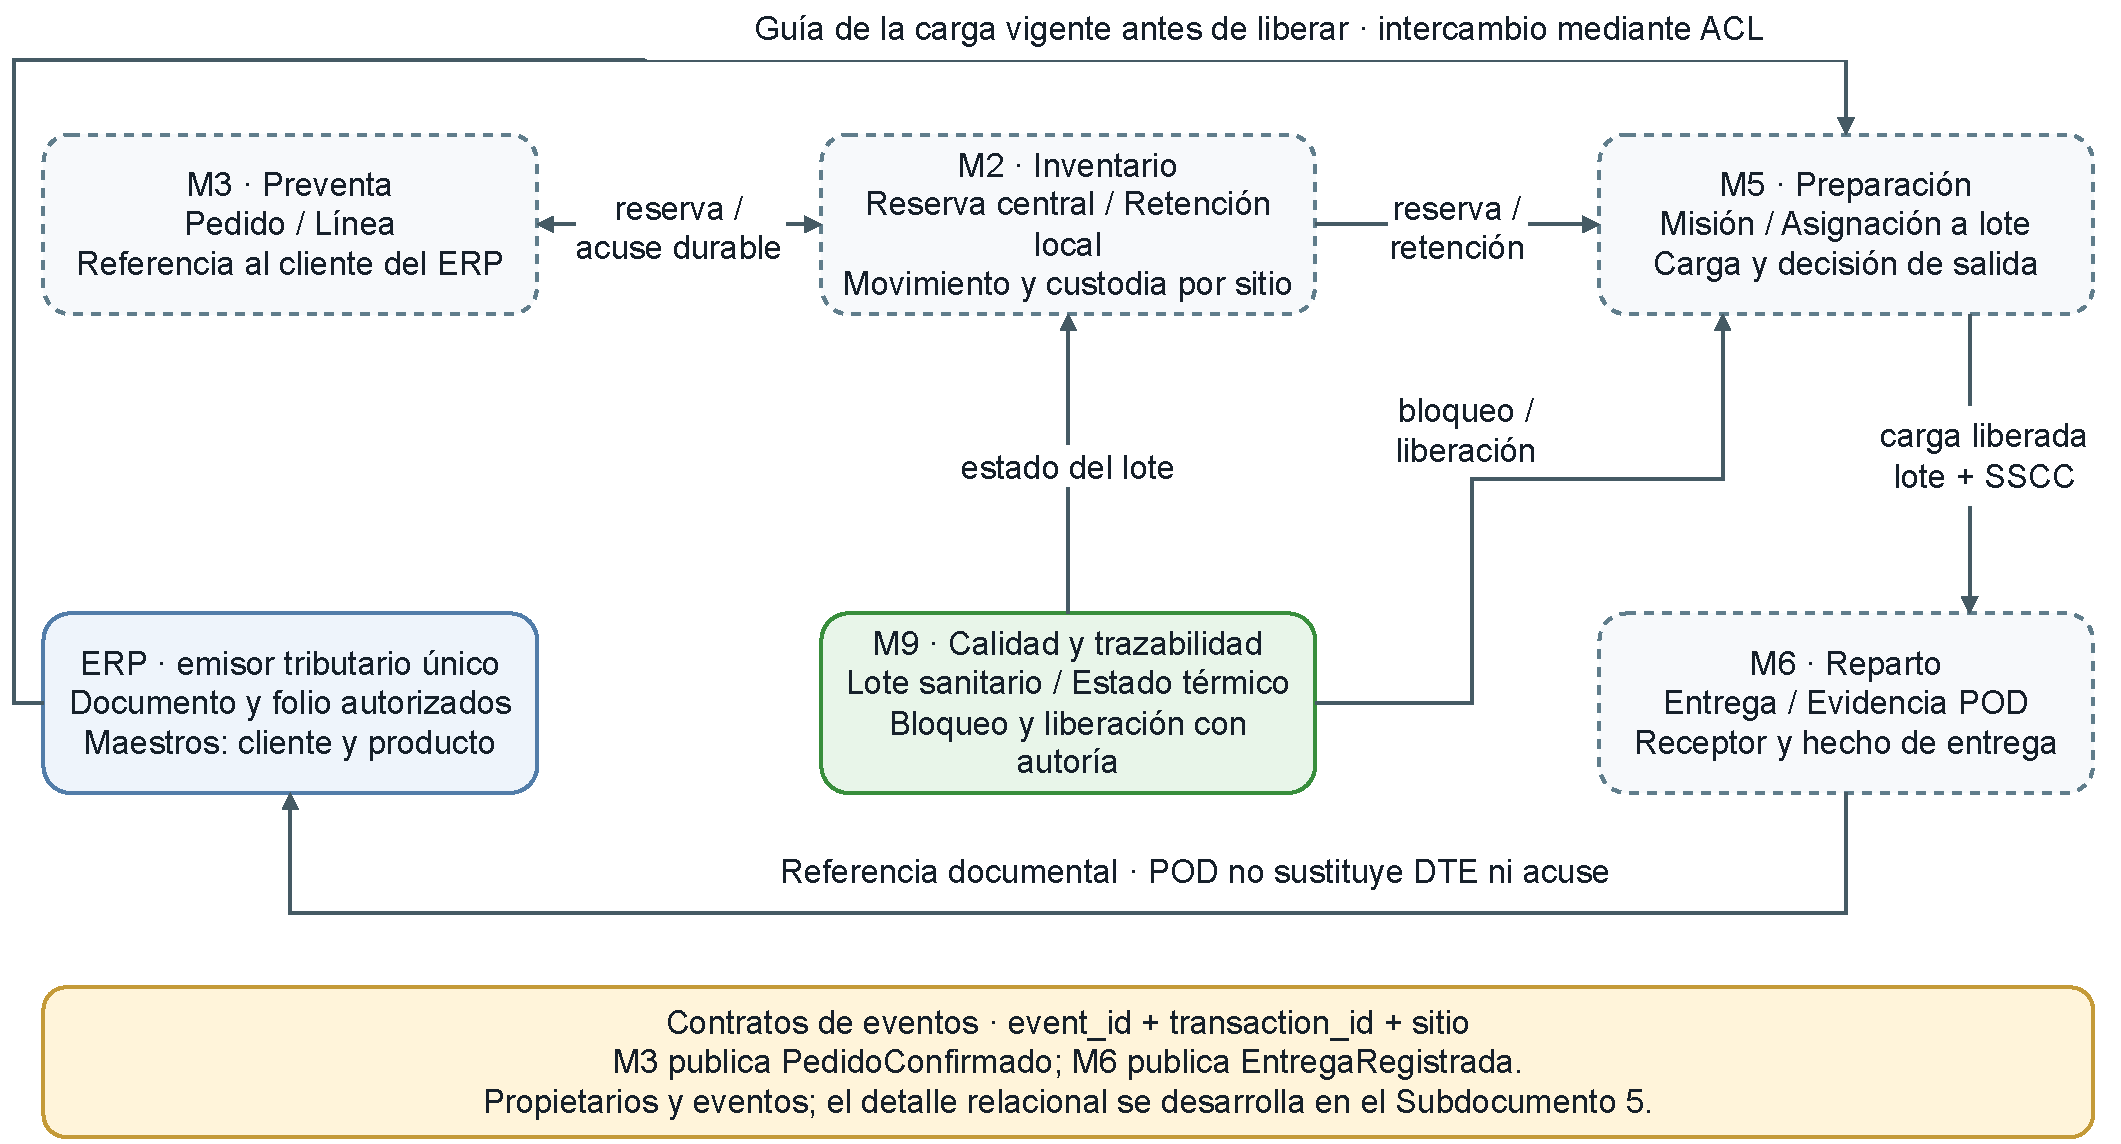
\includegraphics[width=\linewidth,height=0.83\textheight,keepaspectratio]{figuras/logica/complementarias/ARQL-18_Dominio_responsabilidades.pdf}
  \captionof{figure}{Dominio lógico: entidades, módulos responsables y eventos}
  \label{fig:arql-18}
\end{center}

{\footnotesize Fuente: elaboración propia de LafroX.\par}
\end{anexohorizontal}

M3 administra el pedido y sus líneas utilizando la referencia autorizada del cliente del ERP; M2 administra reserva, retención y movimientos por sitio; M5 enlaza misión y asignación a lote con la carga; M9 gobierna el estado sanitario, y M6 registra la entrega y su evidencia. El ERP conserva la emisión tributaria y los maestros autorizados. Los contratos del Anexo 4-A asignan un productor único a cada evento: M3 publica \texttt{PedidoConfirmado} y M6, \texttt{EntregaRegistrada}; compartir el proceso Laravel no permite que otro módulo escriba sus datos privados.

La línea de pedido se asigna a un lote identificado por GTIN y lote del proveedor; los movimientos con SSCC conservan la cadena de custodia hasta la entrega. La entrega vincula la evidencia de recepción y el folio de la guía que el ERP emitió antes del traslado. Un pedido aún puede no tener entrega, y una entrega puede registrar más de una evidencia o un rechazo parcial; los estados conservan el identificador de origen y las cardinalidades se verifican en el modelo del Subdocumento 5. Las flechas de esta vista representan colaboración y contratos; no son claves foráneas ni conexiones directas con bases de datos. El POD no sustituye al DTE ni al acuse del receptor.
